\documentclass[11pt]{article}
\usepackage[margin=1in]{geometry}
\usepackage[T1]{fontenc}
\usepackage[utf8]{inputenc}
\usepackage{lmodern}
\usepackage{amsmath,amssymb}
\usepackage{graphicx}
\usepackage{float}
\usepackage{framed}
\usepackage{booktabs,array,calc}
\usepackage{listings}
\usepackage{caption}
\usepackage[section]{placeins}
\usepackage{microtype}
\usepackage[hidelinks]{hyperref}
\usepackage{bookmark}
\usepackage{xurl}

\urlstyle{same}
\hypersetup{
  pdftitle={Machine Learning Approaches to Identify Security-Sensitive Hotspots in Code},
  pdfauthor={Sahil Sanghvi}
}
\setcounter{secnumdepth}{3}
\setlength{\emergencystretch}{3em}
\providecommand{\tightlist}{%
  \setlength{\itemsep}{0pt}\setlength{\parskip}{0pt}}
\captionsetup{font=small,labelfont=bf}
\newenvironment{architecturebox}
  {\par\medskip\noindent\begin{minipage}{\linewidth}\begin{framed}}
  {\end{framed}\end{minipage}\par\medskip}
\lstset{
  basicstyle=\ttfamily\footnotesize,
  breaklines=true,
  columns=fullflexible,
  keepspaces=true,
  showstringspaces=false
}
\makeatletter
\def\fps@figure{htbp}
\makeatother

\title{Machine Learning Approaches to Identify Security-Sensitive Hotspots in Code}
\author{
  Sahil Sanghvi\\
  {\small Microsoft Azure Security}\\
  {\small \href{mailto:sahilsanghvi@microsoft.com}{\texttt{sahilsanghvi@microsoft.com}}}
}
\date{February 26, 2026}

\begin{document}
\maketitle

\begin{abstract}

This paper demonstrates an application of specialized machine learning
models that reliably identify security-sensitive operations in code and
deliver meaningful cost and operational utility advantages compared to LLM alternatives 
while maintaining classification performance.
The models achieve 74.6\% precision, 77.5\% recall, and 80.1\%
accuracy in human-labeled experiments as well as a 95.42\% precision rate in
modified usage during real-world testing, enabling reliable detection of
privileged operations in previously unseen codebases. This subjective
task has applications for developers implementing security improvements,
security engineers reviewing unseen codebases, and organizational
security efforts at scale. I start by constructing a labeled dataset
using AST-derived representations and a multi-pass LLM pipeline, then
train and evaluate multiple machine learning model architectures
individually and in ensembles. Finally, I validate real-world
applicability by conducting a human-labeled alignment experiment and
demonstrating generalization and operational value. The results
show that building custom models is an efficient and practical method to
identify security-sensitive code that significantly outperforms LLMs in terms of
cost and operational utility, and provides a mechanism that materially improves
security implementation and review workflows at scale.

\noindent

\emph{Keywords}: Security, Machine Learning, Synthetic Data Generation,
Binary classification, Code-as-Data, Sequence Modeling, Security
Automation, Detection Automation, Audit Logging

\end{abstract}

\section{Introduction}\label{introduction}

My team in Microsoft Azure Security is responsible for securing a massive 
software portfolio that spans thousands of Azure offerings. 
Challenges presented by this scale are not unique and are frequently discussed 
in the security community. Thus, we need to find appropriate
methods of automation and standardization to provide security assurance
to vast portfolios. One such method is identifying security ``hotspots'' in
an application's source code, which is valuable to several stakeholders
including application developers and security engineers. Finding and
securing these hotspots has implications for breach prevention, audit
logging, and detailed security review. Thus, an automated method of
finding this code would enable better scaling and effectiveness of many
kinds of proactive security activity.

However, it is difficult to perform this search correctly at scale.
Security-sensitive operations do not neatly fit into patterns and often
depend on context and intent. The task requires a deep understanding of
the code implementation, what other code it interacts with, and a
background in security assessment.

This project demonstrates a method to reliably locate these
security-relevant hotspots by training purpose-built machine learning
models on AST-derived code representations using synthetic data labels.
These models efficiently and effectively predict the probability that a
given piece of code is security-sensitive. Furthermore, it shows that
the custom models meaningfully outperform LLMs for this task in cost
and utility because they deliver deterministic and repeatable
predictions, maintain substantially higher precision and accuracy in evaluations, and operate with computational overhead orders of magnitude
smaller. These characteristics make them far more suitable for
large-scale security workflows, where false-positive triage cost,
reproducibility, latency, and efficiency matter alongside raw
classification metrics.

This paper starts by describing the problem statement and framing it into three
research questions in Section 2, then explains the methodology to answer
these questions in Section 3. It then discusses measurement and evaluation,
future work, threats to validity, and computing efficiency compared to
LLMs in Section 4.

\subsection{Origins \& Related Work}\label{related-work}

This project started from a prototype built during a 2024 company
hackathon at Microsoft. It was inspired by, and uses some techniques
from, a paper called \emph{Where Shall We Log?} (Li et al. 2021), which
used binary classification to compute block-wise predictions of where
general-purpose logging statements (debugging, performance, errors)
should be placed. This paper builds on that predictive approach by applying
similar parsing techniques, but using different models and approaches
tailored to predict security-sensitivity. It also demonstrates an LLM-based
synthetic data pipeline and the system's effectiveness through evaluation 
experiments and real-world testing.

\section{Problem Statement}\label{problem-statement}

\subsection{Research Questions}\label{research-questions}

This paper attempts to answer the research questions below, in
pursuit of the overarching goal of training a machine learning model to
reliably classify security-sensitive code. The first question attempts
to solve the problem using an LLM; the latter two are predicated on
building a purpose-built ML model that would be better than the LLM in
terms of quality and cost.

\subsubsection*{RQ1. How do we develop a dataset of code labeled with security-sensitivity?}\label{rq1.-how-do-we-develop-a-dataset-of-code-labeled-with-security-sensitivity}
\addcontentsline{toc}{subsubsection}{RQ1. How do we develop a dataset of code labeled with security-sensitivity?}

No dataset could be located (as of late 2024) that labeled various
portions of application code as security-sensitive or not. Generating
such a dataset would require significant amounts of domain expert
effort, as even small codebases can contain thousands of blocks of code
when parsed as ASTs.

However, large language models (LLMs) have been shown to be effective at
many different problems that take code as input. Can an LLM effectively
identify whether code is security-sensitive, based on the definition
above?

\subsubsection*{RQ2. What information is most useful in predicting security-sensitivity of code?}\label{rq2.-what-information-is-most-useful-in-predicting-security-sensitivity-of-code}
\addcontentsline{toc}{subsubsection}{RQ2. What information is most useful in predicting security-sensitivity of code?}

Source code exposes many different forms of information, such as control
flow graphs, variable names, etc. (Li et al. 2021) identified 3 vectors
that could be extracted from a piece of code: the semantic, syntactic,
and fused vectors. The semantic vector represents the naming of objects
(functions, variables, etc.), syntactic represents the code structure
(for loop, method declaration, etc.), and fused combines both. All these
vectors are ordered, preserving the ordered nature of the code. Which
vector or combination of vectors is useful to identify
security-sensitive code?

\subsubsection*{RQ3. What model architecture is most useful in predicting security-sensitive code?}\label{rq3.-what-model-architecture-is-most-useful-in-predicting-security-sensitive-code}
\addcontentsline{toc}{subsubsection}{RQ3. What model architecture is most useful in predicting security-sensitive code?}

Binary classification is a general task with many different forms of
solution implementation, including random forests, convolutional neural
networks, etc. Given the vectors from RQ2 as input, which
architecture(s) are the best at performing security-sensitivity binary
classification?

\subsection{Prerequisites}\label{prerequisites}

\subsubsection{Definition of Security-Sensitivity}\label{definition-of-security-sensitivity}

The definition of security-sensitivity is context and organization
dependent and hence inconsistently subjective. Generalized frameworks
may exist, but every organization has nuances related to its operations
and obligations that inform its policies on the subject. For this
project, a definition of security-sensitivity was written based on the 
author's organizational and domain experience, and informed by the 
feedback of colleagues and teammates. It
drew inspiration from internal processes and guidance on security
reviews and audit logging. Security-sensitive code is thus defined as 
direct implementations of operations relevant
to an application's security (which is, by definition, subjective),
including but not limited to:

\begin{itemize}
\item
  Manipulating secrets, identities, and certificates.
\item
  Authenticating and authorizing users and identities, modifying
  authorization groups and hierarchies.
\item
  Modifying application configuration, whether that may be through
  configuration files, in-memory settings, environment variables, or
  something else.
\item
  Modifying Azure resources, which may be an operation as simple as
  creation or as nuanced as updating firewall rules.
\item
  Edge cases and errors that are specifically relevant to the
  application's security, which is subjective and requires an
  understanding of the codebase and application.
\item
  Constructing and invoking externally influenced network requests,
  especially when done in a security-relevant context.
\end{itemize}

These may sound simple at first, but they are nuanced and subjective
categories. It is insufficient to define lists of commonly used APIs to
look for, as the API signatures frequently change and do not account for
custom implementations, or code that is only security-sensitive in the
unique context of one application.

The challenge is predicting where these operations occur in code, while
ignoring benign operations such as reading and writing application data
or performing business logic. Additionally, it was decided to always consider
test cases as being benign. While that might sound obvious, it is something the models
would have to be trained to recognize even if security
functionality was being tested.

\subsubsection{Scope of Input}\label{scope-of-input}

The code used as input in this project is internal C\# source code from
repos in a large internal Azure DevOps instance.

\section{Methodology}\label{methodology}

\subsection{Developing a Labeled Dataset}\label{developing-a-labeled-dataset}

\subsubsection{Parsing and Pre-Processing Code}\label{parsing-and-pre-processing-code}

To develop a dataset for this project, a large volume of code was collected
and parsed into the vectors described in RQ2. Each vector was paired
with a Boolean label (generated in the next section) indicating whether
the vector represented a security-sensitive operation. The scope of input was limited
to Microsoft-owned C\# code from a large internal
Azure DevOps Project. This was due to both the ease of access to that
project and the wide variety of codebases and applications within it to
choose from.

From this project, 22 C\# repositories were selected at random. Each
repository was filtered to .cs files, and each file was parsed using
Python's tree-sitter library into abstract syntax trees (ASTs).

An AST represents code as a hierarchical tree of nodes; the root node is
the entire file, and each child node represents one part of the parent
node, down to leaf nodes representing primitives. Each node represents
some exact subset of the code (e.g. bytes 22 to 49). Nodes always have a
type defined by the language grammar; some examples of node types in C\#
are block, if\_statement, method\_declaration, identifier, and
else\_clause. The block node type represents a logical block of C\# code
(enclosed by curly braces).

The ASTs were used to identify block-type nodes. Following the methodology
used by (Li et al. 2021), these block nodes were ``stretched back'' to
include all preceding code from the start of the containing method,
which are hereafter referred to as ``Cascaded Nodes''. This stretching process enables the
cascaded node to contain useful information about what came before the
block but within the same method, reflecting the sequential nature of
code.

\begin{framed}
\noindent\textbf{Example: Sequence Extraction}

\vspace{2mm}
\noindent Code:

\begin{lstlisting}[language={[Sharp]C}]
private static ExampleProcessor StringProcessor(this FirstArgType arg)
{
    string myString...
\end{lstlisting}

\vspace{2mm}
\noindent Syntactic Sequence:

\begingroup
\small\ttfamily\raggedright
\noindent
{[}method\_declaration local\_declaration\_statement
variable\_declaration...{]}
\par\endgroup

\vspace{2mm}
\noindent Semantic Sequence:

\begingroup
\small\ttfamily\raggedright
\noindent
{[}exampl process string process first arg typ arg my string\ldots{]}
\par\endgroup

\vspace{2mm}
\noindent Fused Sequence:

\begingroup
\small\ttfamily\raggedright
\noindent
{[}method\_declaration exampl process string process first arg typ arg
local\_declaration\_statement variable\_declaration my string...{]}
\par\endgroup
\end{framed}

Each cascaded node is then parsed into three types of sequences.
Starting with a depth-first-search (DFS) traversal of the cascaded node,
we obtain a sequence of the contained AST nodes (from the node
representing the beginning of the method, up to the last node within the
current block). This sequence is filtered to keep nodes that are either
the identifier type, or have a type containing ``expression'',
``statement'', or ``declaration''. The text of the identifier type nodes
is then split into words (assuming Pascal Case casing) and stemmed using
the nltk.PorterStemmer utility to create the semantic sequence. The
other kept node types themselves are the syntactic sequence. The fused
sequence is the combination of the two, preserving order.

After parsing each repository into cascaded nodes, it was obvious that
the dataset was dominated by a few large repositories with much more
than 10,000 cascaded nodes, which would bias models trained on it. To
reduce this effect, the largest repositories were subsampled to a
maximum of 8000 cascaded nodes. This number was chosen to balance the
need to keep the smaller repos from being drowned out while also
retaining the variety and influence that the larger repos had. Some
ended up with slightly less than 8000 due to non-systemic parsing or
processing errors in subsequent steps after subsampling.

\subsubsection{Synthetic Data Labeling using LLMs}\label{synthetic-data-labeling-using-llms}

With the sequence extraction complete, the remaining task was to label
each trio of sequences as security-sensitive or not. As described in
preceding sections, this is a subjective task that requires code
comprehension as well as some knowledge of security implementation and
operations. An LLM prompt was written and iterated over several attempts
to complete this task using best practices such as chain of thought,
persona assignment, and iterative prompt engineering. Evaluation between
iterations was done by hand over random samples of the data as no
pre-labeled set existed at the time. At a high level, the prompt (full
text included in Appendix) instructed the LLM to identify privileged
operations that performed security-sensitive actions directly
implemented in the presented code, and to return a Boolean verdict as
well as a short reason. The prompt incorporated chain of thought and
persona assignment to boost effectiveness.

GPT-4o running on Azure OpenAI served as the labeling LLM as it was
state-of-the-art at that time. To increase confidence in the labels,
each code block was labeled three times independently and only
considered to be security-sensitive if the verdict was True every time.
Loosening this requirement to only need a majority of True
verdicts (two out of three) was considered but rejected in favor of
minimizing false positives at the expense of perhaps increasing false negatives. This was
a practical business decision to avoid false-positive fatigue from
security engineers and developers that would triage and act on the
outputs.

After the labeling loop ran for a few days, a dataset was assembled
with the following characteristics (recall that the largest repos were artificially subsampled to a maximum size, explaining
the similar numbers):

\begin{table}[H]
\centering
\small
\caption{SPECIFICATIONS OF THE TRAINING \& VALIDATION PARSED DATASET}\label{tab:1}
\begin{tabular}{@{}
  >{\raggedright\arraybackslash}p{(\linewidth - 6\tabcolsep) * \real{0.1800}}
  >{\raggedleft\arraybackslash}p{(\linewidth - 6\tabcolsep) * \real{0.1700}}
  >{\raggedleft\arraybackslash}p{(\linewidth - 6\tabcolsep) * \real{0.3400}}
  >{\raggedleft\arraybackslash}p{(\linewidth - 6\tabcolsep) * \real{0.3100}}@{}}
\toprule
\begin{minipage}[b]{\linewidth}\raggedright
Repository
\end{minipage} & \begin{minipage}[b]{\linewidth}\raggedleft
Code Blocks
\end{minipage} & \begin{minipage}[b]{\linewidth}\raggedleft
Security-Sensitive\\
Code Blocks\strut
\end{minipage} & \begin{minipage}[b]{\linewidth}\raggedleft
Percentage of Dataset
\end{minipage} \\
\midrule
Repo 1 & 8000 & 2060 & 9.44 \\
Repo 2 & 7998 & 2156 & 9.43 \\
Repo 3 & 7995 & 2601 & 9.43 \\
Repo 4 & 7993 & 2583 & 9.43 \\
Repo 5 & 7992 & 1496 & 9.43 \\
Repo 6 & 7991 & 1596 & 9.43 \\
Repo 7 & 7988 & 1152 & 9.42 \\
Repo 8 & 7952 & 815 & 9.38 \\
Repo 9 & 6996 & 1852 & 8.25 \\
Repo 10 & 3686 & 552 & 4.35 \\
Repo 11 & 2770 & 231 & 3.27 \\
Repo 12 & 2694 & 385 & 3.18 \\
Repo 13 & 1689 & 289 & 1.99 \\
Repo 14 & 1003 & 228 & 1.18 \\
Repo 15 & 610 & 187 & 0.72 \\
Repo 16 & 542 & 145 & 0.64 \\
Repo 17 & 506 & 197 & 0.6 \\
Repo 18 & 204 & 22 & 0.24 \\
\bottomrule
\end{tabular}
\end{table}

Along with this training set, a set of four more repos was also randomly
sourced to set aside for final testing, estimating real-world performance
after the custom models have been fully trained on the
training/validation dataset:

\begin{table}[H]
\centering
\small
\caption{SPECIFICATIONS OF THE PARSED TESTING DATASET}\label{tab:2}
\begin{tabular}{@{}
  >{\raggedright\arraybackslash}p{(\linewidth - 6\tabcolsep) * \real{0.2300}}
  >{\raggedleft\arraybackslash}p{(\linewidth - 6\tabcolsep) * \real{0.1700}}
  >{\raggedleft\arraybackslash}p{(\linewidth - 6\tabcolsep) * \real{0.3000}}
  >{\raggedleft\arraybackslash}p{(\linewidth - 6\tabcolsep) * \real{0.3000}}@{}}
\toprule
\begin{minipage}[b]{\linewidth}\raggedright
Repository Name
\end{minipage} & \begin{minipage}[b]{\linewidth}\raggedleft
Code Blocks
\end{minipage} & \begin{minipage}[b]{\linewidth}\raggedleft
Security-Sensitive\\
Code Blocks\strut
\end{minipage} & \begin{minipage}[b]{\linewidth}\raggedleft
Percentage of\\
Validation Dataset\strut
\end{minipage} \\
\midrule
Test Repo 1 & 2319 & 396 & 29.67 \\
Test Repo 2 & 2255 & 539 & 28.85 \\
Test Repo 3 & 2133 & 375 & 27.29 \\
Test Repo 4 & 1109 & 117 & 14.19 \\
\bottomrule
\end{tabular}
\end{table}

The dataset was complete, and through copious random spot-checking, some
confidence in its quality had been established. Rigorous measurement of the
quality was constrained by the time repo owners could dedicate
to manually evaluating samples of the predictions, and is discussed further
in Section 4.

\vspace{2mm}

\textbf{Clarification on Labeling Criteria.}

During labeling, the LLM prompt's few-shot examples were inadvertently
compromised. The LLM prompt clearly instructed the model to detect code
that directly implemented security-sensitive operations; however, the
two positive few-shot examples used contained cases where it could be
argued the code invoked rather than directly implemented
security-sensitive code. These two examples were also exact duplicates, meaning there was effectively only one positive example.
This discrepancy likely broadened the effective labeling boundary and
pushed the LLM to be more conservative (lean towards false positives,
declaring security-adjacent code as security-sensitive). It also reduced
example diversity but did not materially affect the labeling process
because each code block was labeled independently multiple times using
the effective system prompt with chain-of-thought techniques for better
results.

Testing results using human-labeled data in Section 4 show that the
custom ML models still generalize well despite this example
inconsistency, but this remains an acknowledged limitation of the
original dataset and one that could be addressed in future work (Section 4.3).

\subsection{Predicting Security-Sensitivity of Code}\label{predicting-security-sensitivity-of-code}

With a large, labeled dataset of code blocks and their parsed sequences,
we move to building predictive models. While an LLM was (in
theory) effective at this prediction, it was expected to be unnecessarily complex and costly. Based on contemporary research,
a few different architecture types are explored in
this section.

Each model was trained using the dataset described in the previous
section, splitting by repo into a larger training set and the smaller
validation set. The testing set was left aside to be used in final
real-world evaluation, after the model hyperparameters and architectures
had been decided. To evaluate model performance, binary
accuracy, precision, recall, and AUPRC (area under the precision-recall
curve) were monitored.

Examining the tables in the previous section, it is clear that this dataset has class
imbalance: the proportion of positive samples (18-22\% across training,
testing, and validation) is significantly smaller than the proportion of
negative samples. Class imbalance is a common problem in binary
classification tasks, and well-known methods are used in the below sections
to account for it when training each model type.

Training was done using a single V100 GPU, for 30 epochs where
applicable. Performance metrics for all models are presented in Section 4.

\subsubsection{Long Short-Term Memory (LSTM) Models}\label{long-short-term-memory-lstm-models}

Prior to transformers, LSTM networks were considered state of the art
for language modeling tasks due to their ability to maintain a hidden
state while processing a sequential input one token at a time. The hypothesis was that this architecture would allow the model to recognize and retain evidence of security-sensitive operations in the beginning or middle of sequences, not just the end.

To accomplish this, the following architecture was built using TensorFlow:

\begin{architecturebox}
\noindent\textbf{Model Architecture: Fused Sequence LSTM}

\begin{itemize}
\item
  A vectorizer layer trained on all fused sequences for the dataset.
  This layer serves as the model's vocabulary, assigning each token in
  the sequences to a specific integer ID.
\item
  An embeddings layer, which learns a 512-dimensional representation of
  the meaning of a token.
\item
  An LSTM layer with a hidden state of size 128.
\item
  An LSTM layer with a hidden state of size 64.
\item
  A dropout layer (used during training only to prevent overfitting).
\item
  A dense neural network layer with 64 neurons.
\item
  A second dense neural network layer with 64 neurons.
\item
  A dense neural network layer with 16 neurons.
\item
  A single output neuron that outputs a probability (using sigmoid
  activation).
\end{itemize}
\end{architecturebox}

When training this model, class weights determined by the training
dataset were used to scale up loss for positive samples and scale down
loss for negative samples, addressing the class imbalance issue. The
Adam optimizer was used with a learning rate of 0.001 and binary focal
cross-entropy loss with \((\alpha = 0.25,\ \gamma = 2.0)\) default
values, which also helps mitigate class imbalance instead of the typical
binary cross-entropy loss.

The input sequences were truncated to the last 400 tokens to
prevent the model from being overwhelmed by mostly empty sequences
filled with padding tokens, as the longest sequences were around 2000
tokens but were an extreme minority. Almost all sequences were naturally
400 tokens or less, so this prevented an architecture decision from
being made based on a small number of outliers.

\begin{figure}
\centering
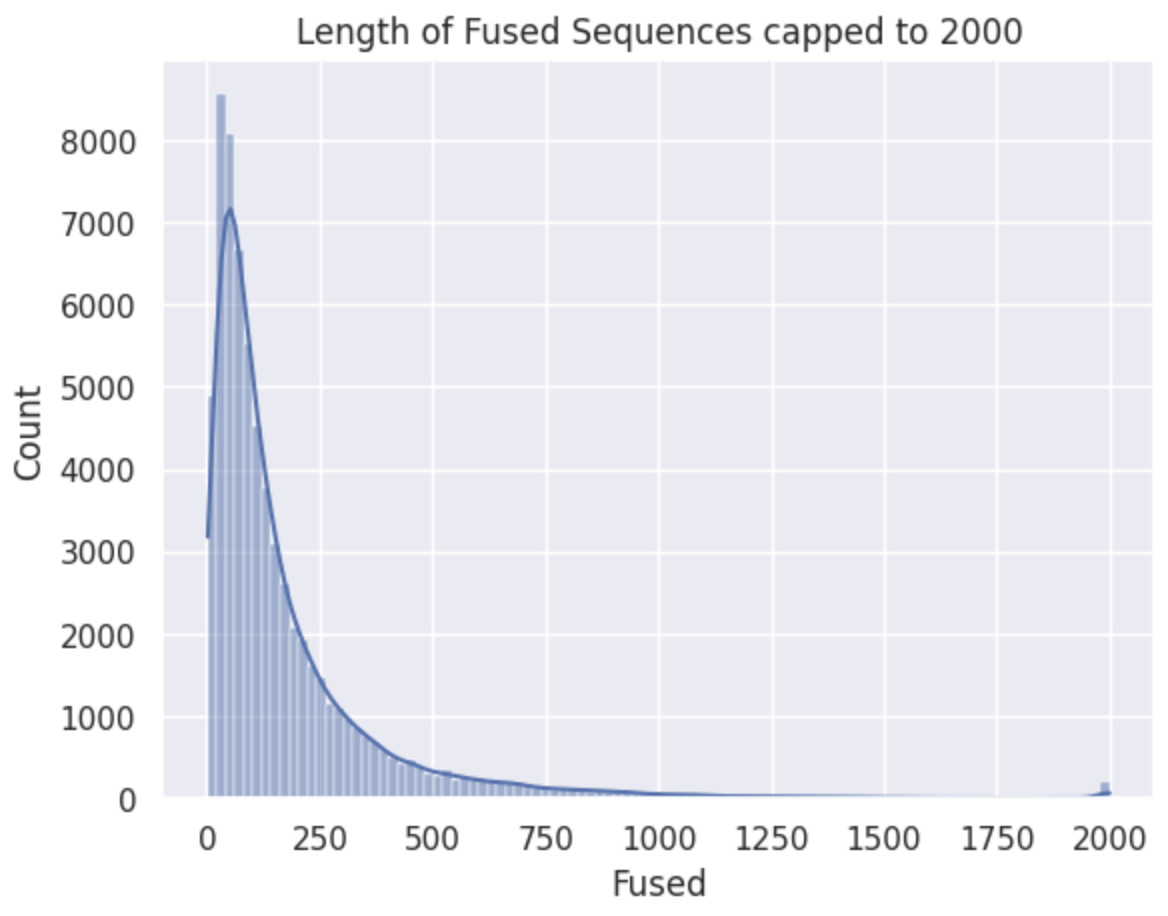
\includegraphics[width=0.5903\linewidth,height=\textheight,keepaspectratio,alt={The distribution of fused sequence lengths has a tall peak close to 50, with a very long tail.}]{./media/image1.png}
\caption{The distribution of fused sequence lengths has a tall peak close to 50, with a very long tail.}\label{fig:1}
\end{figure}

Parameters and hyperparameters including the model layer parameters,
learning rate, and batch size were varied to get the best results,
using a V100 GPU for 30 epochs as mentioned earlier.

Along with an LSTM trained on fused sequences, another LSTM was also
trained using only semantic information. As seen below, it is noticeably
less complex than the fused LSTM, likely due to the more straightforward
relations between tokens in the sequences:

\begin{architecturebox}
\noindent\textbf{Model Architecture: Semantic Sequence LSTM}

\begin{itemize}
\item
  A vectorizer layer trained on all semantic sequences in the dataset.
  This layer serves as the model's vocabulary, assigning each token in
  the sequences to a specific integer ID.
\item
  An embeddings layer, which learns a 256-dimensional representation of
  the meaning of a token.
\item
  An LSTM layer with a hidden state of size 128.
\item
  A dropout layer (used during training only to prevent overfitting).
\item
  A dense neural network layer with 64 neurons.
\item
  A dense neural network layer with 16 neurons.
\item
  A single output neuron that outputs a probability (using sigmoid
  activation).
\end{itemize}
\end{architecturebox}

This time, the semantic sequences were truncated to the last 300 tokens,
for a similar reason as the fused sequences above. The same
optimizer, loss function, and class weighting as above were used,
addressing the class imbalance issue, and the hyperparameters were
similarly experimented with to get the final model.

Both finalized models performed decently well on the testing data, with
the Fused sequence model having a slight edge in AUPRC and Recall while
the Semantic sequence model had the edge in Precision and Binary
Accuracy. Full testing metrics are presented in Section 4 for
comparison with other model types.

\subsubsection{Convolutional Neural Networks (CNNs)}\label{convolutional-neural-networks-cnns}

Convolutional neural nets are most famous for image processing but have
been shown to be effective for language processing tasks as well (Kim
2014). This architecture tested whether inferring over distinct overlapping
windows of the input sequences would better identify security-sensitive
snippets in a broader sequence. A CNN was trained with Fused sequences
using the following architecture:

\begin{architecturebox}
\noindent\textbf{Model Architecture: Fused Sequence CNN}

\begin{itemize}
\item
  A vectorizer layer trained on all fused sequences for the dataset.
  This layer serves as the model's vocabulary, assigning each token in
  the sequences to a specific integer ID.
\item
  An embeddings layer, which learns a 512-dimensional representation of
  the meaning of a token.
\item
  A Convolution1D layer with 64 filters and a kernel size of 6 to
  operate on small slices of the sequence at a time.
\item
  A MaxPooling1D layer with window size 2 that retains only the
  strongest signal from each window.
\item
  A dense neural network layer with 32 neurons.
\item
  A single output neuron that outputs a probability (using sigmoid
  activation).
\end{itemize}
\end{architecturebox}

As with the LSTM models, class imbalance was addressed by using class weights
to scale loss and using binary focal cross entropy loss instead of
regular binary cross entropy loss. The fused sequences were again
truncated to the most recent 400 tokens, and different batch sizes,
learning rates, and model layer parameters were then experimented with to
identify the best architecture.

The final fused CNN had the best testing AUPRC and Recall out of all the
models, but a lackluster Precision score. Specific metrics are compared 
with other model types in Section 4.

\subsubsection{Random Forests (RF)}\label{random-forests-rf}

Random Forests are large collections of many randomly initialized
individual decision trees. The decision trees are all fully independent,
and their outputs are aggregated to form the final prediction of the
forest. While LSTMs are aware of input sequence ordering and CNNs
loosely take advantage of it, the Random Forest model is truly
order-agnostic. It simply takes the sequence as a large, unordered
collection of tokens.

This model tested whether the collection of tokens was
more informative than the order in which they appeared. As Section 4
will show, this yielded higher precision but lower recall than the
sequential models, which does partially support the hypothesis.

One related and notable difference between this model and the previous
ones is the method of vectorization. In previous models, the
tokens were translated into numerical identifiers, and then into embeddings representing
their meaning. However, for decision trees, the model learns which token
features are most valuable for prediction by branching the tree based on
which token features correlate most strongly with the true output they are
trying to predict. Therefore, TF-IDF was used, which
assigns each token a value based on its inverse frequency in the
dataset. This gives higher weight to rarer tokens, which often carry
more signal for modeling tasks, but also introduces the possibility of
overweighting typos or unique identifiers. To address this pitfall, the
TF-IDF vectorizer's maximum size was limited to the 12000 most frequent
tokens in the dataset, ignoring any remainders. This was a na\"{i}ve
mitigation but effective in practice, as we see in the results in
Section 4.

\begin{architecturebox}
\noindent\textbf{Model Architecture: Fused Sequence Random Forest}

\begin{itemize}
\item
  A TF-IDF vectorizer layer trained on all fused sequences for the
  dataset, with a maximum feature set of size 12000.
\item
  A Random Forest with 248 estimators (trees), minimum sample split of
  16, and using Gini Impurity to measure splits.
\end{itemize}
\end{architecturebox}

Unlike the neural models in the past sections which were tuned by hand
adjusting hyperparameters like batch size and learning rate, Gaussian
optimization was used to automatically find the best
parameters for the random forest by searching across the defined ranges
of each parameter. The ranges were 100 to 600 estimators, minimum sample
split between 2 and 20, with and without bootstrapping, and Gini or
log-loss criterion.

The final random forest had a surprisingly competitive validation
Precision score and AUPRC, with mediocre Recall. Full testing
metrics are presented in Section 4 for comparison with other model
types.

\subsubsection{Support Vector Machines (SVMs) and Logistic Regression Models}\label{support-vector-machines-svms-and-logistic-regression-models}

Some other model architectures were also attempted along with the three
above, but there was not enough promising progress to pursue them beyond
prototyping:

\begin{itemize}
\item
  Support Vector Machines (SVMs) operate by effectively finding
  multi-dimensional decision boundaries. One was trained on TF-IDF
  representations of the fused sequences using Gaussian optimization to
  find good hyperparameters. This did not yield promising results, and
  the line of research was ended.
\item
  Logistic Regression models are perhaps the simplest binary models and
  were almost certainly too simple for the problem at hand. One was
  prototyped using the TF-IDF vectors of the fused sequences and
  cross-validation to improve hyperparameter selection. This did not
  yield promising results either.
\end{itemize}

\subsubsection{Ensembling Strategy}\label{ensembling-strategy}

With four models that all performed decently well (Fused LSTM, Semantic
LSTM, Fused CNN, and Fused RF), there were now four probabilities for any given
input representing how likely it was to be security-sensitive. Two ways
of combining these predictions (commonly referred to as ensembling) were
evaluated: taking the mean and training a small ``ensembler'' neural
network. The first is a simple mathematical operation; for the latter,
small network architectures with one to three dense layers with 4 to 8
neurons (plus an output neuron) each were tested.

The plot below shows the precision-recall curves for all the individual
models as well as the two ensembling approaches. A curve that bulges out
further indicates better performance of the model across many different
decision thresholds. It was clear that ensembling provided a significant
benefit, and that ensembling by a simple mean was the better approach.

\begin{figure}
\centering
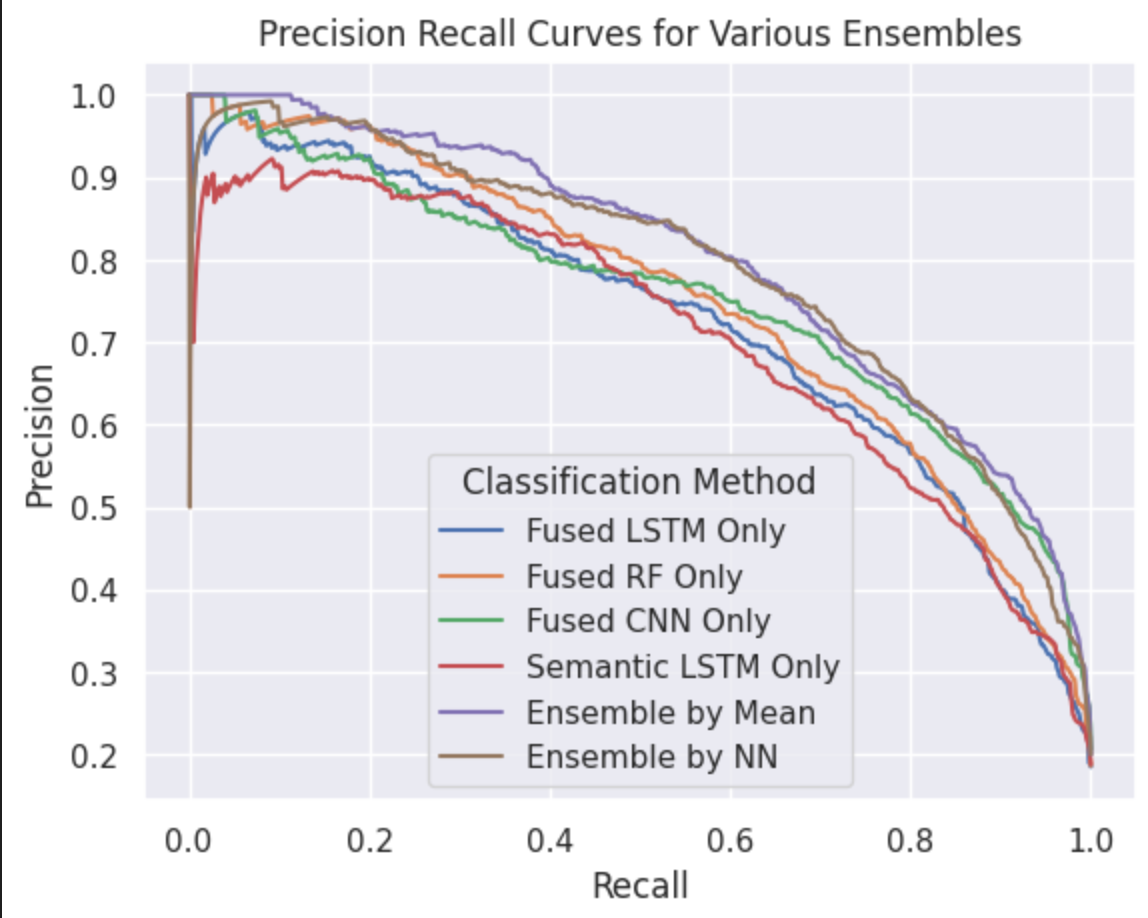
\includegraphics[width=0.59831\linewidth,height=\textheight,keepaspectratio,alt={A precision-recall plot showing the precision-recall curves of each of the 4 individual models as well as the 2 ensembling methods. The 2 ensembling methods are visually better by a little bit. }]{./media/image2.png}
\caption{Precision-Recall Curves for different models and ensembles show the benefit of ensembling.}\label{fig:2}
\end{figure}

\section{Discussion \& Results}\label{discussion-results}

\subsection{System Evaluation}\label{system-evaluation}

The system was evaluated at multiple points during its lifecycle.
Training and validation metrics were evaluated as the models were built,
followed by metric evaluation on the testing set, which was entirely
unseen and not used for any model architecture choices. Following that,
alignment was evaluated by conducting an alignment experiment
using human-labeled data instead of LLM-labeled data. Finally, real-world 
performance metrics were evaluated to get further insight into the quality of the results.

\subsubsection{Testing Metrics}\label{testing-metrics}

Once the models were declared complete using training and validation data, performance on the entirely unseen
testing dataset was evaluated to ensure good generalization. Those testing metrics are presented below.

\begin{table}[htbp]
\centering
\small
\caption{TESTING DATASET METRICS OF VARIOUS MODELS}\label{tab:3}
\begin{tabular}{@{}
  >{\raggedright\arraybackslash}p{(\linewidth - 8\tabcolsep) * \real{0.3400}}
  >{\raggedleft\arraybackslash}p{(\linewidth - 8\tabcolsep) * \real{0.1800}}
  >{\raggedleft\arraybackslash}p{(\linewidth - 8\tabcolsep) * \real{0.1600}}
  >{\raggedleft\arraybackslash}p{(\linewidth - 8\tabcolsep) * \real{0.1600}}
  >{\raggedleft\arraybackslash}p{(\linewidth - 8\tabcolsep) * \real{0.1600}}@{}}
\toprule
\begin{minipage}[b]{\linewidth}\raggedright
Model/Ensemble
\end{minipage} & \begin{minipage}[b]{\linewidth}\raggedleft
Binary Accuracy
\end{minipage} & \begin{minipage}[b]{\linewidth}\raggedleft
Precision
\end{minipage} & \begin{minipage}[b]{\linewidth}\raggedleft
Recall
\end{minipage} & \begin{minipage}[b]{\linewidth}\raggedleft
AUPRC
\end{minipage} \\
\midrule
Fused LSTM & 85.86\% & 58.43\% & 78.21\% & 0.7267 \\
Semantic LSTM & 86.30\% & 60.27\% & 73.23\% & 0.7088 \\
Fused CNN & 86.19\% & 58.59\% & 83.18\% & 0.7547 \\
Fused Random Forest & 88.52\% & 78.62\% & 51.02\% & 0.7497 \\
\textbf{Ensemble} by Mean & 88.51\% & 66.12\% & 76.03\% & 0.8020 \\
\textbf{Ensemble} by Neural Network & 89.52\% & 70.88\% & 72.32\% &
0.7879 \\
\bottomrule
\end{tabular}
\end{table}

\subsubsection{Alignment Experiment}\label{alignment-experiment}

Evaluating the system using the testing dataset in the previous section
gives confidence that the models have not overfit to the
train/validation set. It tells us that the models perform well on unseen
data sourced in the exact same way. However, that data sourcing may
potentially be biased because it is synthetic data labelled by an LLM.
Any biases the LLM had in how it decided whether to consider the code as
security-sensitive would be present in both datasets. Thus, it was now
necessary to perform an alignment experiment with human-labeled data to
identify any such bias.

7 new repos that were not linked to any previous stage of
development were selected to perform this testing.

The exact procedure was as follows:

\begin{enumerate}
\def\labelenumi{\arabic{enumi}.}
\item
  The models were run over the entire repo, and then a
  random sample of at least 2\% of blocks up to a maximum of 60 blocks
  was selected for human labeling. This sample was a uniform random sample,
  independent of the outputs. While larger samples would have been
  preferable, asking busy engineers to voluntarily spend time labeling data acted as a practical limitation on the maximum sample size.
\item
  Once the sample of blocks was selected, the prediction values were hidden and
  the service engineer was asked to join a call. The call began with a set of
  written instructions covering what we considered to be security-sensitive,
  which were also explained verbally following a similar script.
  During the call the service engineer manually assigned a Boolean label
  to each block in the sample. Minimal input was provided beyond the existing instructions on how to decide if
  things were security-sensitive, and the service engineer used their
  knowledge about what the exact purpose of the code was to make a
  decision. This is not the most ideal way to obtain labels but was the
  most practical way to get the data needed in a timely manner from
  busy professionals. Biasing responses was avoided as much as possible, though this is difficult to fully guarantee.
\item
  The human labels were then compared to the model outputs (using a standard
  decision threshold of 0.5 to decide when the model output should count
  as a positive or negative prediction). This plot shows the raw metrics
  of each sample, with each group representing one repository. Repository names are intentionally omitted.

  \begin{figure}[H]
  \centering
  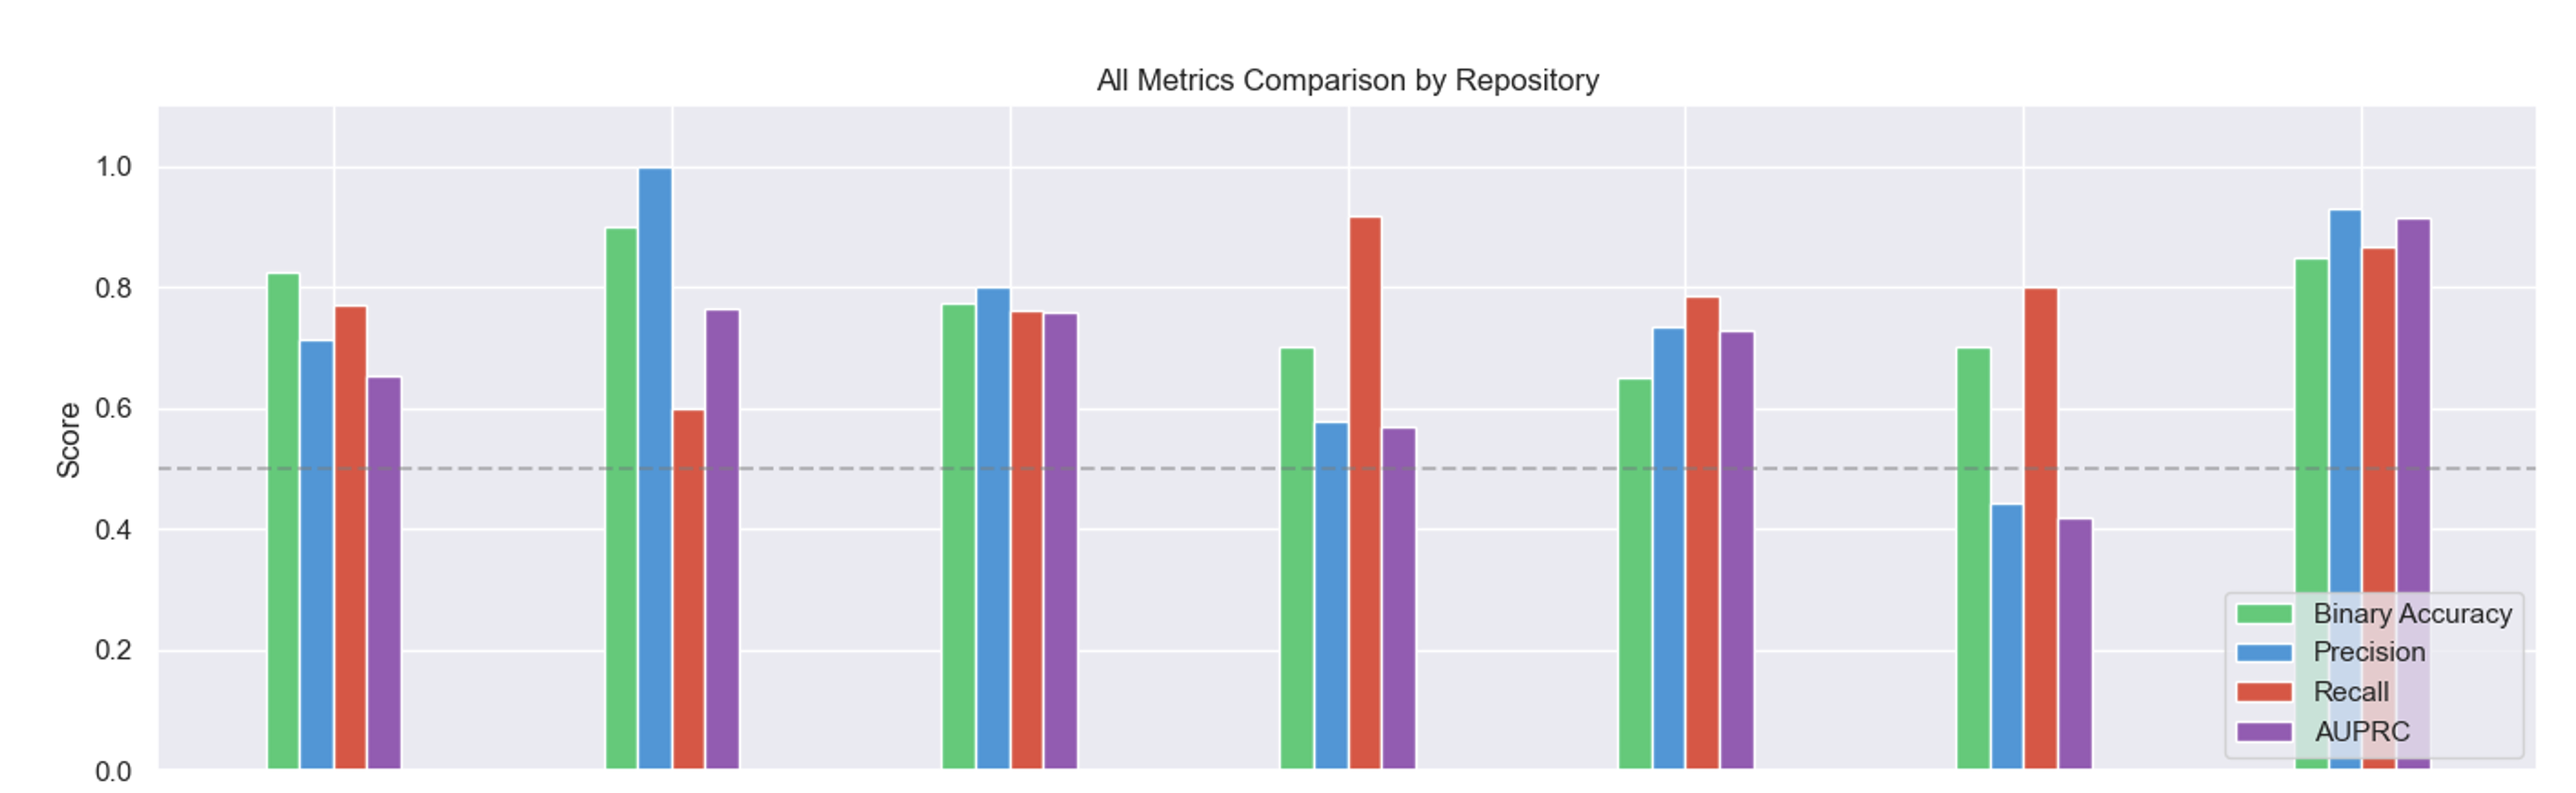
\includegraphics[width=0.93873\linewidth,height=\textheight,keepaspectratio]{./media/image3.png}
  \caption{Metrics calculated over each small, labeled sample.}\label{fig:3}
  \end{figure}

  The second repository from the right appears to be a low outlier.
  Further investigation into this repo revealed that it was an internal security application. 
  It may be the case that the concentration of security-related language in the semantics of 
  the code was conflated
  with security-sensitive operations, though more investigation is
  required.
\item
  Once all the blocks in the random sample were labeled, a bootstrap simulation was performed \((b = 200)\), sampling repeatedly with
  replacement to simulate gathering many more labeled samples.
\item
  Binary accuracy, precision, recall, and AUPRC were calculated for each simulated sample. The distribution of values
  for each metric across samples was used to calculate both a sample mean and a confidence
  interval using the percentile method \((\alpha = 0.025)\). These two
  descriptors represented an estimate of that metric over the entire
  repo, not just the small labeled sample.
\item
  The sample mean of each metric was then combined across the seven repos
  by taking a mean weighted by the size of each repo. This estimates the performance of the models on \emph{any} block in
  \emph{any} of these repos, and serves as evidence of 
  generalization and real-world alignment since these repos were
  entirely unseen and labeled by humans.
\end{enumerate}

\begin{table}[H]
\centering
\small
\caption{EXTRAPOLATED METRICS OVER REPOS IN EXPERIMENT}\label{tab:4}
\begin{tabular}{@{}
  >{\raggedright\arraybackslash}p{(\linewidth - 4\tabcolsep) * \real{0.2400}}
  >{\raggedleft\arraybackslash}p{(\linewidth - 4\tabcolsep) * \real{0.3400}}
  >{\raggedleft\arraybackslash}p{(\linewidth - 4\tabcolsep) * \real{0.4200}}@{}}
\toprule
\begin{minipage}[b]{\linewidth}\raggedright
Metric
\end{minipage} & \begin{minipage}[b]{\linewidth}\raggedleft
Bootstrap Mean Value
\end{minipage} & \begin{minipage}[b]{\linewidth}\raggedleft
95\% Confidence Interval
\end{minipage} \\
\midrule
Binary Accuracy & 80.1\% & {[}73.6, 86.0{]} \\
Precision & 74.6\% & {[}60.2, 85.9{]} \\
Recall & 77.5\% & {[}63.7, 88.1{]} \\
AUPRC & 0.668 & {[}0.560, 0.787{]} \\
\bottomrule
\end{tabular}
\end{table}

\begin{figure}[H]
\centering
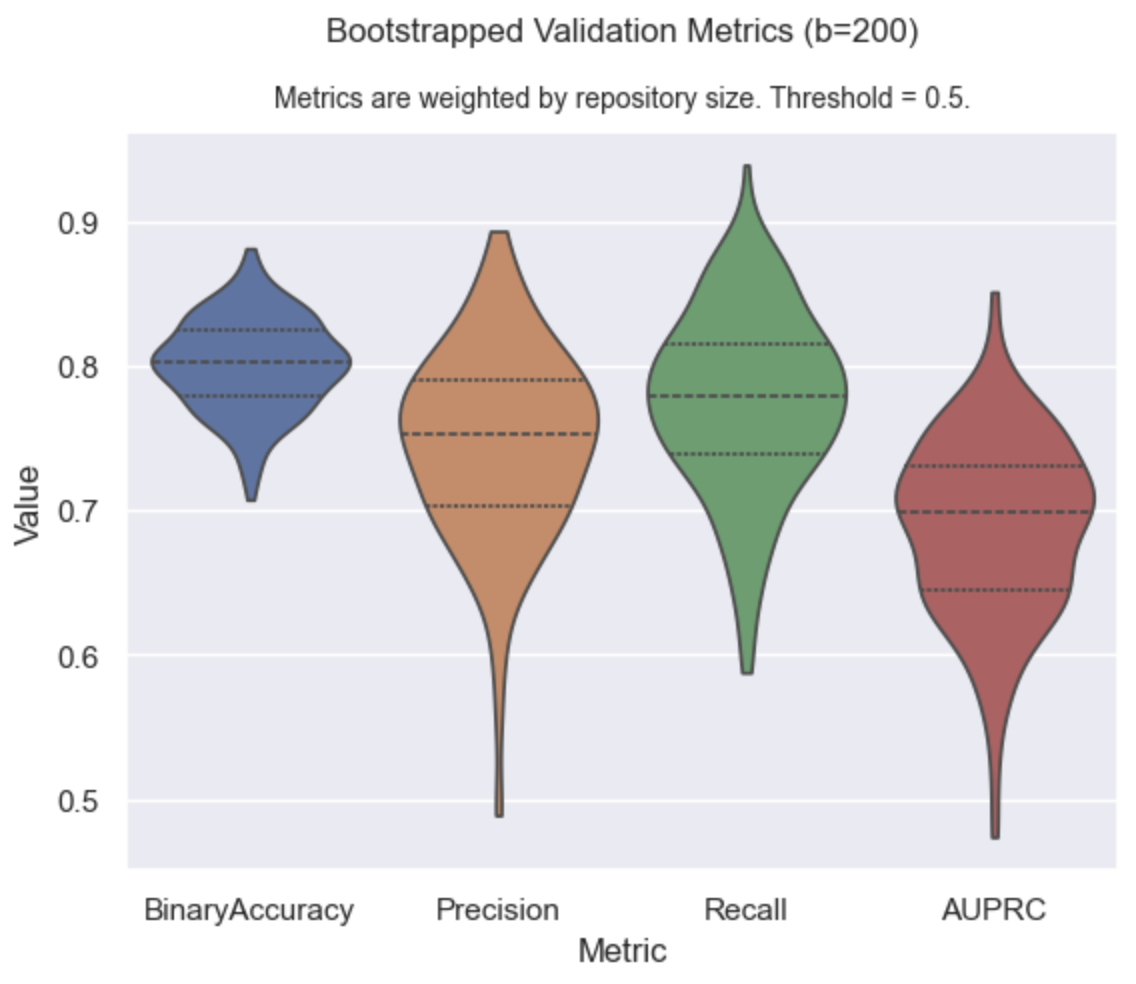
\includegraphics[width=0.6\linewidth,height=\textheight,keepaspectratio,alt={A violin plot showing the bootstrap distributions of the weighted aggregated metrics.}]{./media/image4.png}
\caption{A violin plot showing the bootstrap distributions of weighted aggregated metrics.}\label{fig:4}
\end{figure}

\textbf{Discussion.}

While the seven repos in scope were not a true random sample 
(they were owned by teams that had working relationships with my team),
they reflected real production code and were not selected systematically or with intent to positively affect
system evaluation. The extrapolated metrics based on
human-labeled data show much higher precision, slightly higher
recall, and lower binary accuracy than the testing dataset performance
in the last section. The metrics suggest moderate to good alignment with human judgement on the task, 
and the proximity of results between testing data
and human-labeled data suggests generalization to unseen repos, subject
to the biases noted above. When combining these results with the testing
set metrics in the previous section and real-world testing metrics in the
next one, the evidence that these models have generalized to the task
becomes stronger.

\subsubsection{Real-World Testing}\label{real-world-testing}

This tool is one of many complementary approaches used to increase 
audit logging coverage in Azure, and was tested in the real world by 
incorporating it into an internal review process. 

This real-world usage had a few key differences:

\begin{itemize}
\item
  Instead of being delivered at the block level, results were aggregated
  (via a simple mean) at the method level. Methods are easier for
  engineers to work with than the individual blocks within them.
  Each method thus has a prediction representing the probability that
  code in that method is security-sensitive. This approach may seem like
  it would ignore methods with one small security-sensitive part, but
  because blocks are nested, many of the blocks are classified as
  security-sensitive even in these cases.
\item
  A threshold was selected to cut off results by reviewing the method
  predictions near it to optimize for delivering more signal than noise.
  This allows selection of a threshold which delivers the most
  actionable insights for users, but is also an acknowledged source of bias that makes
  the usage metrics skew positively. The threshold is typically in the
  range {[}0.75, 0.8{]}.
\item
  A list of all methods flagged as being security-sensitive
  was delivered. A shortcoming of this approach is that it only allows measurement of true and false positives; no one reviewed
   the negatives. Additionally, service
  teams may be biased to agree with ``the security team'' when it is asserted
  that code is security-sensitive.
\end{itemize}

In the real-world test, 41 repositories containing
over 155,000 methods were scanned. Of those, 3499 methods were flagged as
security-sensitive. When operating at scale, this intelligent filtering
would provide great operational value in prioritizing security effort.
Code owners triaged 612 flags and agreed with 95.42\% of them (an
operational precision rate of 95.42\%).

\begin{figure}[H]
\centering
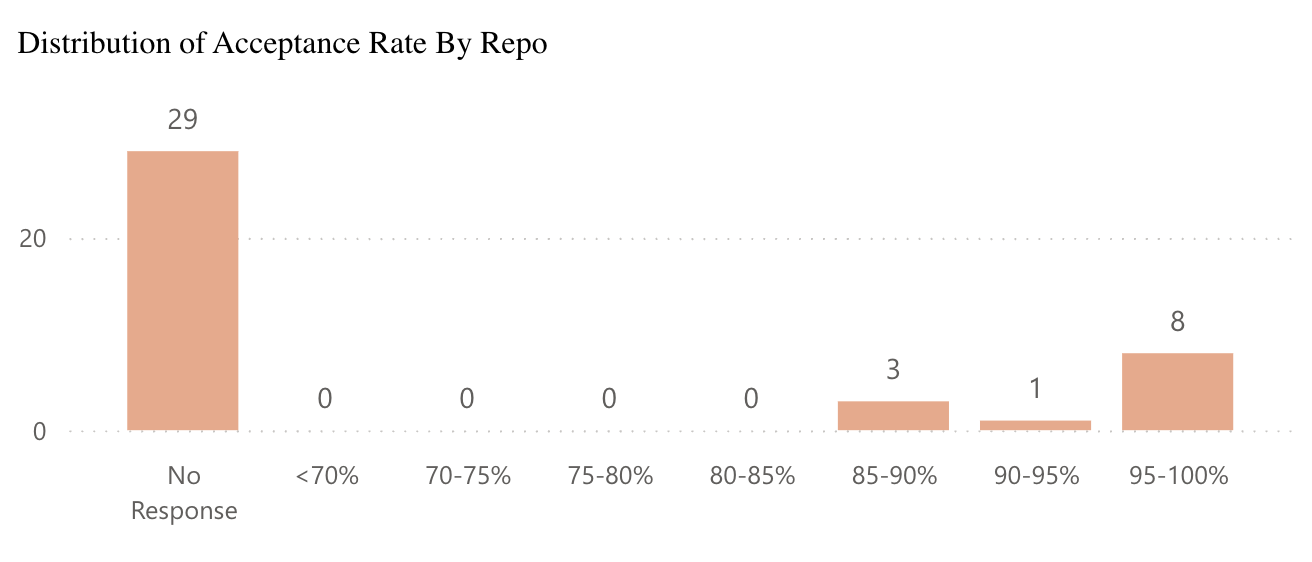
\includegraphics[width=1\linewidth,height=\textheight,keepaspectratio]{./media/image5.png}
\caption{A distribution of acceptance rates by repo. All triaged repos accept over 85\% of flagged methods.}\label{fig:5}
\end{figure}

Several teams took these findings a step further by using them to
make tangible improvements in their code, resulting in over 120 new audit
logging statements in valuable and relevant locations. Additionally,
my colleagues found this work useful in prioritizing their manual code
review during security reviews. Anecdotally, a reviewer looked at the
most security-sensitive prediction for a service and found a critical
vulnerability in that code, which directly led to a detection improvement 
to discover hundreds of similar high severity vulnerabilities acrosss the estate!

While this real-world testing naturally introduces upward bias in measurement
for the reasons explained above, the testing dataset metrics and
human-labeled alignment experiment in previous sections provide
additional evidence that the models are genuinely robust and effective.

\subsection{Research Question Results}\label{research-question-results}

\subsubsection*{RQ1: How do we develop a dataset of code labeled with security-sensitivity?}\label{rq1-how-do-we-develop-a-dataset-of-code-labeled-with-security-sensitivity}
\addcontentsline{toc}{subsubsection}{RQ1: How do we develop a dataset of code labeled with security-sensitivity?}

As we saw in earlier sections, this task was accomplished using
a mix of deterministic and non-deterministic tools. Deterministic
tools like tree-sitter were used to parse the code, break it up into logical
blocks, and extract consistent and informative sequences. An LLM prompt was
then written and refined with few-shot examples, chain-of-thought
prompting, and persona assignment that did a decent job of labeling code
as security-sensitive as judged by random spot-checking.

The quality of the LLM tagging is evaluated in two
ways. Firstly, the human-labeled data gathered for the validation
experiments is also used to evaluate the quality of the LLM tagging:

\begin{figure}[H]
\centering
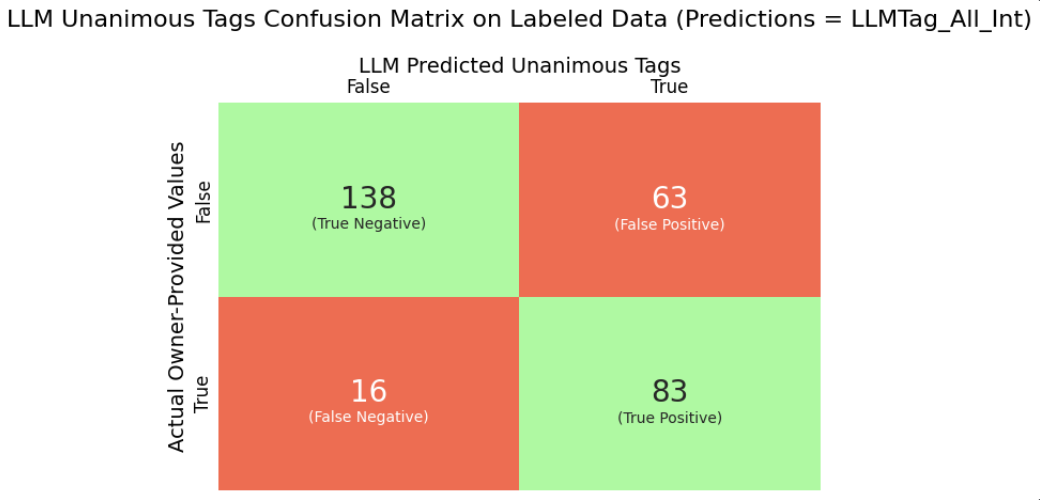
\includegraphics[width=0.60444\linewidth,height=\textheight,keepaspectratio,alt={A confusion matrix showing the performance of the LLM tagging over the human labeled set.}]{./media/image6.png}
\caption{A confusion matrix showing the performance of the LLM tagging over the human labeled set.}\label{fig:6}
\end{figure}

Manually computing the metrics for this confusion matrix yields a binary
accuracy of 73.67\%, precision of 56.84\%, and recall of 83.84\%.
Bootstrapped confidence intervals constructed using the same methods as
before are provided in Table 5 below. These are not particularly strong
metrics but do indicate moderate efficacy. Based on this sample it is
much more likely for an incorrect label to be a false positive rather
than a false negative, meaning that the LLM tagging was overly cautious
in its decisions, because it was more likely to falsely claim code was
security-sensitive. This is most likely attributable to the inadvertent
discrepancies in the few-shot examples described in Section 3.1.2.

The second indication that the LLM tagging was of acceptable quality is
that the downstream custom models work
well, as shown by the testing dataset metrics, human-label alignment experiment, and the real-world test metrics.

In fact, because the LLM's confusion matrix in Figure~6 is computed over
the same previously unseen human-labeled dataset used in the evaluation
experiments, it shows that the purpose-built models meaningfully
outperform the LLM in real-world utility. In this task context, utility
refers to achieving high accuracy and precision at minimal
false-positive triage cost, with reproducible results and low
computational demands.

\begin{table}[htbp]
\centering
\small
\caption{LLM COMPARED TO CUSTOM MODELS}\label{tab:5}
\begin{tabular}{@{}
  >{\raggedright\arraybackslash}p{(\linewidth - 8\tabcolsep) * \real{0.1600}}
  >{\raggedleft\arraybackslash}p{(\linewidth - 8\tabcolsep) * \real{0.1600}}
  >{\raggedleft\arraybackslash}p{(\linewidth - 8\tabcolsep) * \real{0.2200}}
  >{\raggedleft\arraybackslash}p{(\linewidth - 8\tabcolsep) * \real{0.2400}}
  >{\raggedleft\arraybackslash}p{(\linewidth - 8\tabcolsep) * \real{0.2200}}@{}}
\toprule
\begin{minipage}[b]{\linewidth}\raggedright
Metric
\end{minipage} & \begin{minipage}[b]{\linewidth}\raggedleft
LLM:\\
Metric Value\strut
\end{minipage} & \begin{minipage}[b]{\linewidth}\raggedleft
LLM:\\
95\% Confidence Interval\strut
\end{minipage} & \begin{minipage}[b]{\linewidth}\raggedleft
Custom Models:\\
Bootstrap Mean Value\strut
\end{minipage} & \begin{minipage}[b]{\linewidth}\raggedleft
Custom Models:\\
95\% Confidence Interval\strut
\end{minipage} \\
\midrule
Binary Accuracy & 73.67\% & {[}70.0, 77.7{]} & 80.1\% (+6.4\%) &
{[}73.6, 86.0{]} \\
Precision & 56.84\% & {[}48.9, 64.1{]} & 74.6\% (+17.7\%) & {[}60.2,
85.9{]} \\
Recall & 83.84\% & {[}76.7, 90.1{]} & 77.5\% (-6.3\%) & {[}63.7,
88.1{]} \\
\bottomrule
\end{tabular}
\end{table}

Even though LLMs were effective enough to generate a large initial
dataset, their behavior was insufficient for the operational
requirements of this task at scale. When evaluating both approaches on
the same human-labeled dataset, the LLM achieves lower
precision (comparing both the bootstrap means and the confidence
intervals), which is important to note given the cost of a false
positive in this context. Additionally, LLM labels are not guaranteed to
be consistent and repeatable across runs, providers, and batches in
practice; all important qualities for a security detection to have.

On the other hand, the purpose-built models learn a specific token-level
decision boundary from their structured code-derived inputs, enabling
deterministic and repeatable classification with much higher
precision. The precision boost is especially valuable in the context of
this task, where false positives translate to real triaging cost for
security engineers and application developers. The custom models avoid
the substantial latency, throughput, and inference costs associated with
LLMs, which scale poorly when thousands of blocks must be classified.

This shows that even with the same misaligned labeling signal from the
prompt examples, the specialized models achieve higher precision and
accuracy than the LLM on the same human-labeled dataset. Even though the
LLM achieves a higher recall score, the custom models deliver materially
stronger real-world precision-favored utility while requiring only a
small fraction of the computational resources, which is expanded on in
Section 4.4. This classification stability, cost efficiency, and
precision advantage combined make it clear that the custom models are a
more reliable and scalable solution for this security-sensitivity
classification task and operational context.

\subsubsection*{RQ2. What information is most useful in predicting security-sensitivity of code?}\label{rq2.-what-information-is-most-useful-in-predicting-security-sensitivity-of-code-1}
\addcontentsline{toc}{subsubsection}{RQ2. What information is most useful in predicting security-sensitivity of code?}

Looking at the 4 models in the ensemble, we see that three use the fused
sequences (both semantic and syntactic information) and one uses only
semantic information. The semantic-only model did not systematically
outperform nor underperform the fused models. This indicates that while
semantic information alone is enough to make predictions about the
security sensitivity of code, the addition of syntactic information
likely increases robustness of prediction.

Intuitively, this makes sense: the semantic information is the names of
variables, methods, and other objects, which usually indicate their
purpose and relevance. Syntactic information helps understand the
relation between all the semantic tokens.

It should be noted that the syntactic node-type allow list was overly
restrictive, which presents an opportunity for future improvement (Section 4.3).

\subsubsection*{RQ3. What model architecture is most useful in predicting security-sensitive code?}\label{rq3.-what-model-architecture-is-most-useful-in-predicting-security-sensitive-code-1}
\addcontentsline{toc}{subsubsection}{RQ3. What model architecture is most useful in predicting security-sensitive code?}

Two of the four final models use the LSTM architecture. This is not
particularly surprising, as LSTMs were a popular and capable choice
for language modeling tasks prior to the rise of transformer models. It is likely the LSTM's ability to maintain that long
short-term memory that enables better predictions over long sequences,
regardless of the position of the security-sensitive code within the
sequence.

\subsection{Opportunities for Improvement}\label{next-steps-opportunities-for-improvement}

This project demonstrated promise, but there are still opportunities for improvement in any future work:

\begin{enumerate}
\def\labelenumi{\arabic{enumi}.}
\item
  Consuming a larger dataset containing more business verticals and code languages.
  It would be useful to compare a multi-lingual model to language-specific models.
\item
  Improving dataset quality by fixing issues around parsing the code into
  sequences, including:

  \begin{enumerate}
  \def\labelenumii{\alph{enumii}.}
  \item
    Integrating large portions of syntactic information which were being
    ignored due to an overly restrictive allowlist when filtering
    out meaningful syntactic nodes (e.g. a method call) from
    insignificant ones (e.g. an opening parenthesis).
  \item
    Significantly improving the splitting of semantic tokens,
    handling several types of common casing (Pascal, camel, snake,
    etc.), numbers, and jargon or special words (e.g. ``OAuth2'' instead
    of ``O'', ``Auth'', ``2'').
  \end{enumerate}
\item
  Increasing confidence in the synthetic LLM labels by
  modifying the prompt and examples to align the LLM more closely to expectations
  and demonstrate desired behavior across different languages. This includes 
  resolving the discrepancies in few-shot examples discussed in Section 3.1.2.
\item
  Evaluating additional model types, such as a
  transformer-encoder model.
\end{enumerate}

\subsection{Computational Performance Advantage}\label{computational-performance-advantage}

The introduction claimed that these models outperformed costly and
complex LLMs in both quality and cost at this security-sensitivity
classification task. Section 4.2.RQ1 shows how this claim is true for
quality, and this section will justify the claim for cost.

The purpose-built models are smaller, cheaper, faster, and run locally.
The Fused LSTM has 19.8 million parameters occupying 75MB of memory, and
the Fused CNN is almost the same in both counts. The relatively simple
Semantic LSTM only has 9.9 million parameters, occupying 38MB.

OpenAI has not released parameter counts for GPT-4o, but it is
well-known that it is not suitable for running on average consumer
hardware or devices. Even GPT-OSS20b, which is considered to be more
accessible to run locally, uses 21 billion parameters and requires at
least 12GB of memory. These requirements are multiple orders of
magnitude larger than the smaller models built in this project.

Indeed, in operational use the models frequently run locally on standard business
laptops (e.g. Surface Laptops, ThinkPads) which do not usually have a
GPU. Large repos with several thousand files and tens of thousands
of methods complete analysis in two minutes or less even on CPU-only
devices. For example, the models classified a repo with 2560 blocks in
13 seconds (approximately 196 classifications per second) on a MacBook Pro
whereas an LLM, even if running locally, would struggle to classify more
than 1 block (1 request) per second. If we consider remote providers,
the dataset tagging pipeline required approximately 3 seconds to send
and receive a request for a single block when using Azure OpenAI with a
high quota (780 requests per minute). Even if the LLM were to run in
parallel by batching blocks, quality would likely decrease to the point
of being unusable with a batch size nearing 600 for equivalent
throughput. Parallelizing the requests themselves could decrease the runtime, but would require extremely high quotas and would still incur higher costs and latency. This means the custom models are more efficient at this task
through many lenses such as electricity, time, or hardware requirements.

Preliminary measurements of time and cost differences were calculated on
a set of five varied repositories used for a business analysis of this
project. To accomplish this, the following assumptions grounded in
experiences and observations from this project were used:

\begin{enumerate}
\def\labelenumi{\arabic{enumi}.}
\item
  It takes approximately 3 seconds per LLM label on Azure OpenAI using
  sophisticated prompt engineering and high-effort reasoning settings.
  This does not include transient error retries, rate limiting, or other
  factors that might cause delays.
\item
  Using an LLM to classify a method requires a 600-token instruction
  prompt, which aligns with the prompt used in this project, and results in
  an average output length of 100 tokens to allow for light chain of
  thought reasoning and an output label with a short explanation. The
  600-token prompt would be cached input as it is repeated in each
  request.
\item
  An average method length is 200 tokens, which aligns with the sequence
  lengths seen in the dataset. The method would be non-cached input as
  it changes in each request.
\end{enumerate}

Using the above assumptions and current Azure OpenAI billing rates at
the time of writing, the following cost and time estimates are obtained.

\begin{table}[htbp]
\centering
\small
\caption{ESTIMATED LLM CLASSIFICATION COSTS}\label{tab:6}
\begin{tabular}{@{}
  >{\raggedright\arraybackslash}p{(\linewidth - 10\tabcolsep) * \real{0.1200}}
  >{\raggedleft\arraybackslash}p{(\linewidth - 10\tabcolsep) * \real{0.1400}}
  >{\raggedleft\arraybackslash}p{(\linewidth - 10\tabcolsep) * \real{0.1800}}
  >{\raggedleft\arraybackslash}p{(\linewidth - 10\tabcolsep) * \real{0.2200}}
  >{\raggedleft\arraybackslash}p{(\linewidth - 10\tabcolsep) * \real{0.1700}}
  >{\raggedleft\arraybackslash}p{(\linewidth - 10\tabcolsep) * \real{0.1700}}@{}}
\toprule
\begin{minipage}[b]{\linewidth}\raggedright
Repo
\end{minipage} & \begin{minipage}[b]{\linewidth}\raggedleft
Method Count
\end{minipage} & \begin{minipage}[b]{\linewidth}\raggedleft
Cached Input Cost
\end{minipage} & \begin{minipage}[b]{\linewidth}\raggedleft
Non-Cached Input Cost
\end{minipage} & \begin{minipage}[b]{\linewidth}\raggedleft
Output Cost
\end{minipage} & \begin{minipage}[b]{\linewidth}\raggedleft
Total Cost
\end{minipage} \\
\midrule
Repo A & 917 & \$0.10 & \$ 0.32 & \$1.28 & \$1.70 \\
Repo B & 33027 & \$3.57 & \$11.56 & \$46.24 & \$61.36 \\
Repo C & 2957 & \$0.32 & \$1.03 & \$4.14 & \$5.49 \\
Repo D & 241 & \$0.03 & \$0.08 & \$0.34 & \$0.45 \\
Repo E & 556 & \$0.06 & \$0.19 & \$0.78 & \$1.03 \\
\bottomrule
\end{tabular}
\end{table}

The total estimated cost of LLM analysis on this set is \$70.04. In
comparison, the custom model ensemble was deployed on an Azure Function
(Premium SKU) and cost \$2.78 per day, regardless of the number of repos scanned. Running the analysis multiple
times on multiple days demonstrated stability in this price.

\begin{table}[htbp]
\centering
\small
\caption{ESTIMATED RUNTIME COMPARISON}\label{tab:7}
\begin{tabular}{@{}
  >{\raggedright\arraybackslash}p{(\linewidth - 8\tabcolsep) * \real{0.1200}}
  >{\raggedleft\arraybackslash}p{(\linewidth - 8\tabcolsep) * \real{0.1500}}
  >{\raggedleft\arraybackslash}p{(\linewidth - 8\tabcolsep) * \real{0.2100}}
  >{\raggedleft\arraybackslash}p{(\linewidth - 8\tabcolsep) * \real{0.2400}}
  >{\raggedleft\arraybackslash}p{(\linewidth - 8\tabcolsep) * \real{0.2800}}@{}}
\toprule
\begin{minipage}[b]{\linewidth}\raggedright
Repo
\end{minipage} & \begin{minipage}[b]{\linewidth}\raggedleft
Method Count
\end{minipage} & \begin{minipage}[b]{\linewidth}\raggedleft
Runtime: Local
\end{minipage} & \begin{minipage}[b]{\linewidth}\raggedleft
Runtime:\\
Azure Function\strut
\end{minipage} & \begin{minipage}[b]{\linewidth}\raggedleft
LLM Estimated Runtime
\end{minipage} \\
\midrule
Repo A & 917 & 6 sec & 1 min 28 sec & \textasciitilde46 min \\
Repo B & 33027 & 3 min 43 sec & 50 min 57 sec & \textasciitilde1 day 3.5
hours \\
Repo C & 2957 & 19 sec & 3 min 54 sec & \textasciitilde2.5 hours \\
Repo D & 241 & 2 sec & 27 sec & \textasciitilde12 min \\
Repo E & 556 & 5 sec & 41 sec & \textasciitilde27 min \\
\bottomrule
\end{tabular}
\end{table}

The total estimated runtime, without factoring in rate limiting,
transient errors, etc., of an LLM at this task is 1 day and 7.5 hours.
By comparison, the custom model ensemble evaluates the same inputs in
less than 5 minutes locally and approximately 1 hour on a minimal cloud
deployment. The cloud runtime can be improved using a higher-powered
compute offering, and further cost and latency analysis is ongoing.

The cost and latency comparison in this section is on equivalent tasks,
as both systems are considered under a requirement of systematic and
guaranteed coverage where every method is assessed. While an LLM-based
implementation could instead use an agentic or heuristic-driven
exploration strategy, preliminary internal comparisons suggest such
approaches lack determinism and coverage on large repositories due to
context window limitations. These effects stem from the sampling-based
generation and bounded context innate to LLMs, rather than
implementation choices. Mitigating these issues would require additional
engineering work to enforce coverage and state retention, which would
increase system complexity, engineering cost, and latency.

These preliminary and limited results suggest that this project
outperforms an LLM solution at the given task in terms of cost
(approximately 25x decrease) and latency (approximately 31.5x decrease
in a minimal cloud deployment) while retaining similar or even better
prediction quality.

\subsection{Threats to Validity}\label{threats-to-validity}

This section assembles and acknowledges the different sources of bias
and error that are mentioned throughout this paper and addresses mitigations against them.

\begin{itemize}
\item
  The LLM prompt few-shot examples were mishandled such that the
  positive examples were duplicates, and it could be strongly argued
  that they are invocations rather than implementations of
  security-sensitive code. The error is mitigated by the system prompt itself (which was correct and used reliable prompting
  strategies), and the real-world test showing an acceptably high precision
  rate (a low precision rate would be an indicator of the overly
  cautious behavior the insufficient examples might elicit).
\item
  The operational metrics likely skew positively due to service teams
  deferring to the judgement of ``the security team'' and me choosing a
  threshold to optimize for actionability. However, the testing dataset and
  human-labeled experiments included many more negative samples than
  positive predictions, and the good performance on those indicates that
  the conclusions are still plausible.
\item
  Human-labeled sample gathering was subject to natural limitations on
  quantity and availability, and the confidence intervals reflect
  resampling of the limited labels available. Still, the intervals and
  bootstrap means are consistent with testing performance and
  real-world metrics, supporting the overall conclusion of strong
  performance.
\end{itemize}

\section{Conclusion}\label{conclusion}

This project shows that security-sensitive code can be reliably
identified using lightweight machine learning models trained on
AST-derived representations, outperforming LLMs in both real-world
utility and cost at this task. It demonstrates practical construction of
a large synthetic dataset, evaluation of several purpose-built model
architectures, and rigorous evaluation through multiple approaches.
These specialized models efficiently surface security-relevant code
hotspots at scale with strong real-world alignment, as proven through
an alignment experiment and real-world testing. This work demonstrates
a potential capability for scalable code classification in service of 
proactive security efforts in large organizations, and illustrates the 
broader opportunity for targeted ML-based tools to meaningfully support robust
development and review practices.

\appendix

\section{Appendix}\label{appendix}

\subsection{LLM Prompt to Tag Code as Security-Sensitive}\label{llm-prompt-to-tag-code-as-security-sensitive}

\textbf{System Prompt}

\begin{lstlisting}
# Task: Privileged Operation Classification in Source Code
- You are a security engineer who specializes in identifying privileged operations *directly* present in source code.
- Privileged operations in source code are *security-sensitive* instructions.
- *Some* examples of privileged operations are:
    - Creating, updating, or deleting user identities
    - Reading, creating, updating, or deleting secrets or certificates.
    - Authenticating or authorizing users to a system, or configuring an authentication and authorization system.
    - Deploys, modifies, upgrades, or deletes an Azure cloud resource or its configuration
    - Changes, or attempts to change, to an application's configuration
- On the other hand, you must *not* falsely identify benign operations as security-sensitive. 
- *Some* benign operations are:
    - Reading non-secret data, like a user's claims, the status of a cloud resource, or data from a database.
    - Logging
    - Converting data types
    - test cases, indicated by attributes like [Fact] and [TestCase] and others, are always benign.
- You must determine whether the code the user provides contains a security-sensitive privileged operation.
    - The code must **directly perform** the privileged operation, not simply refer to entities used in privileged operations.
- Remember that *test cases, indicated by attributes like [Fact] and [TestCase] and others, are always benign!*
### Input and Output Format
- The user will provide you with a snippet of code. It may be incomplete.
- You must determine whether the given code, interpreted strictly as-is, contains a security-sensitive privileged operation.
- Your output should be a JSON object with two properties: reason and verdict.
    - reason is a short phrase or sentence explaining your thought process.
    - verdict is a boolean of whether the code contains a security-sensitive privileged operation.
    - Remember that *test cases are always benign!*
\end{lstlisting}

\textbf{Few-Shot examples have been removed as they contain Microsoft
proprietary source code.} There were 5 few-shot examples, of which 2
were positive and 3 were negative. The inputs were raw code snippets,
and the outputs matched the format described in the prompt.

\newpage
\noindent \textbf{License:} This work is licensed under a Creative Commons Attribution-NonCommercial 4.0 International License (CC BY-NC 4.0).
\begin{thebibliography}{9}

\bibitem{li2021}

Zhenhao Li, Tse-Hsun (Peter) Chen, and Weiyi Shang. 2021. Where shall we
log? studying and suggesting logging locations in code blocks. In
Proceedings of the 35th IEEE/ACM International Conference on Automated
Software Engineering (ASE \textquotesingle20). Association for Computing
Machinery, New York, NY, USA, 361--372.
\url{https://doi.org/10.1145/3324884.3416636}

\bibitem{kim2014}

Kim, Yoon. "Convolutional neural networks for sentence
classification."~\emph{arXiv preprint arXiv:1408.5882}~(2014).

\end{thebibliography}

\end{document}
